\chapter{Apache Kafka}
\label{intro-kafka}

As this thesis is about the implementation of a message broker that correlates
to the functionalities Apache Kafka provide, we describe in the following the
components and functionalities of Apache Kafka in the current state (Version
0.8.2). This shall provide a basis for further comparison (see \ref{survey-broker}) with
more traditional broker systems, which is why won't provide any implementation
specific details in this section but describe the concepts in a higher level of
abstractness instead. Thus, it is also an overview and the initial position of our
own implementation (see \todo{ref}), in which Chapter the implementation
specific aspects will be resolved in detail. 

\section{Background}

Apache Kafka was initially developed at LinkedIn\cite{linkedin} and subsequently
released as an open source project with the Apache Software
Foundation\cite{apachefoundation}. 
\\ \\
Initially at LinkedIn the landscape was overwhelmed by the complexity due to
point-to-point (\ref{intro-messaging-pointtopoint})
pipelines that delivered data to a single destination with no
integration between. Messages were written to aggregated files and then copied
to ETL servers (data integration) and further loaded into data warehousing and batch
processing (\ref{intro-datastream-batchprocessing})
clusters. Thus, this service included the lack of real-time data access which
is---especially for a data driven company that populates activity-driven news
feeds---an essential requirement. In fact, this fragility and complexity of this
pipeline lead to inevitable delays in adding new types of activity data.
Besides the feature wise limitations, also the detection time of operational
problems increased over time due to the ever-increasing pressure on the latency
of the data warehouse processes. This could have been solved with
stream processing systems (\ref{intro-datastream-streamprocessing}) but again, 
due to the lack of any central platform (\ref{intro-datastream-centralplatform})
that can provide continuous data, was not supported at this point.
\cite{goodhope2012building}

First attempts towards a piece of infrastructure (e.g. broker) that can server
stream and batch processing systems were made by experimenting with
ActiveMQ\cite{activemq}. During tests under full production load they ran into
several significant problems. It turned out that if the queue backed up beyond what could
be kept in memory, performance would severely degrade due to heavy amounts of
random I/O. Inefficiencies had to be accepted regarding clustered consumers
requiring duplicating the data for each consumer in a separate queue. Further
difficulties were faced with ActiveMQ's built in persistence mechanism that lead
to very long restart times. 
\todo[inline]{well, reasons are not that overwhelming honestly...}
According to LinkedIn it would have been possible to provide enough buffer to
keep the ActiveMQ brokers above water but would have required hundred servers to
process a subset of activity data. As a result, the decision was made to build a
custom piece of messaging infrastructure targeting high-volume scale-out
deployment and thus serve batch and stream processing systems. 
\cite{goodhope2012building}


\section{Characteristics}
- Zitat: One key feature of Kafka is its functional simplicity. While there is a
lot of sophisticated engineering under the covers, Kafka’s general functionality
is relatively straightforward. Part of this simplicity comes from its
independence from any other applications (excepting Apache ZooKeeper)

\section{Use Cases}
\begin{description}
    \item [Traditional message broker]
    \item [Log aggregation]
    \item [Stream processing] Kafka's strong durability is very useful in the
        context of stream processing
\end{description}

\section{The Log}
\label{intro-kafka-log}
Apache Kafka uses a so-called commit log for managing messages within the
broker. This log has nothing in common with "application logging", as traces of
a software designed for human read. Instead, logs in the context of distributed systems
are designed for programmatic access. Basically it is a simple, append-only data
structure which contains a sequence of records ordered by time whereas each
entry is assigned to an unique number, called offset. Thanks to the strict
ordering inside a log the record offset can be used as timestamp whereas a log
gets decoupled from any time system. \cite{apachekafka} \cite{JK-TheLog}

\begin{figure}[H]
    \centering
    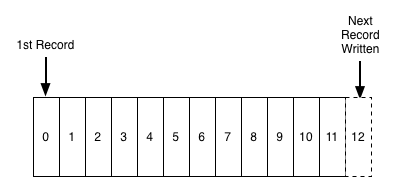
\includegraphics[width=0.4\textwidth]{images/log.png}
    \caption{The  Log \cite{JK-TheLog}}
    \label{fig:the-log}
\end{figure}

Apache Kafka handles a own log for every topic whereas the log contains all
published messages as single records. Compared to traditional messaging systems,
Kafka does not delete a record after consumption, actually it makes no difference
 whether or not they have been consumed. As we see later, every consumer
controls its position of the log by its own. Kafka can hold records within a
defined time window before it deletes the oldest records of the log.
Further more, an additional feature called log compaction can be activated to reduce the amount of messages
which need to be deleted by removing only obsolete records. \cite{apachekafka} \cite{JK-TheLog}

Logs originally come from databases where they are used to for replication
whereas the log includes records of what happened. Every change or update of a
log leads to a new state that represents a version including all the updates
done in past. Describing every replica by the latest log entry it has processed, 
the problem of coordinating states of distributed replicas is getting much easier.
Apache Kafka uses this approach for consumption of messages. Every consumer knows its actual offset and
increases it linearly as it reads messages from the log. The log can be seen as a
re-playable record of history whereas a consumer also can reset to an older
state---by using the offset---to reprocess. \cite{JK-TheLog}

\begin{figure}[H]
    \centering
    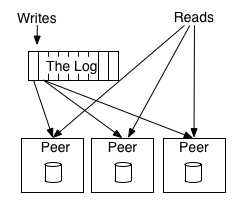
\includegraphics[width=0.4\textwidth]{images/state-machine-replication.png}
    \caption{Peers can sync their state with the log \cite{JK-TheLog}}
    \label{fig:the-log}
\end{figure}

\section{Components}

\subsection{Consumer / Producer}
- consumer / producer grouping

\subsection{Persistance}
Apache Kafka stores all data immediately to a persistent log
(\ref{intro-kafka-log}) 
and therefore relies heavily on the \gls{file system}.
Instead of flushing incoming messages from producers directly to the disks, the
data is stored as a compact byte structure within the \gls{page cache}.
\\ \\
The process of copying the data to the disk is handled by the operating system
that will not only use linear reads and writes \todo{gls} as a pattern for heavy
optimization but also provides read-ahead and write-behind techniques.
The latter will pre-fetch data in large block multiples and group smaller logical
writes into large physical writes. Thus, a SATA RAID-5 of six 7200rpm
disks will achieve a performance of 600MB/s in writes.
\\ \\
As a result of of the mentioned factors of using the file system and relying on
\gls{page cache} leads to the fact that Apache Kafka claims access to all free memory.
Doing so will result in a cache of up to 28-30GB on a 32GB machine. In a default
setup, data is kept in memory for 7 days to provide data required for processing
directly from the memory. This duration should be set according to of one's own
needs. In fact, the memory stays persistent during a restart of the Kafka
service but won't if the server restarts for example. In the latter scenario,
Apache Kafka will restore all data from the disk to the memory.
\cite{apachekafka} \\ \\
One drawback following this model of not immediately writing data to disk can not be
omitted. A small number of messages can be lost in the event of a hard server
failure before messages are transfered to the Kafka brokers or flushed to disk.
\cite{goodhope2012building}

\subsection{Partitioning}
Facing the challenges of large distributed systems, a log must scale well. For
improving scalability and fault tolerance, Kafka can divide a log in multiple
partitions and is a way to parallelize the consumption of the messages, whereas
the total number of partitions in a broker cluster need to be at least the same
as the number of consumers (or producers) in a consumer (or producer) group.

\begin{figure}[H]
    \centering
    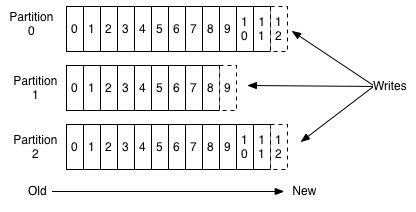
\includegraphics[width=0.5\textwidth]{images/log_anatomy.png}
    \caption{Partitioned Log \cite{apachekafka}}
    \label{fig:the-log}
\end{figure}

Each member---be it on consumer or producer side---will split the burden of
processing the topic between themselves according to the partitioning so that
one member will only be concerned with messages in the partition itself is
assigned to. 

\subsection{Message Delivery}
\label{kafka-message-delivery}
\todo[inline]{kafka = pull based model}
\todo[inline]{kafa's guarantees regarding message delivery}
\subsection{Replication}
To hold the defined guarantees (\ref{kafka-message-delivery}) regarding to system
or network failures, Apache Kafka supports \gls{replication} on the level of log
partitions \todo{ref}. Thereby it can replicate specific topics across a configurable
number of other other Kafka nodes. Every topic has a defined leader node which
is active in normal operation. A leader node can have zero or more followers
which are responsible for replicating the entries of the leader log. The followers
do this by simply act as a normal Kafka consumer of the leader node and
constantly update their own log so that it is identical. Every incoming message
needs to be replicated by every follower node before any other consumer can get
it. A fully replicated message is considered as "commited". This guarantees that
the consumer need not worry about potentially seeing a message that could be
lost if the leader fails. \cite{apachekafka}

\todo[inline]{illustration}

\todo[inline]{zookeeper}

\subsection{Compression}

\subsection{Batching}

%\subsection{The Producer}

%\subsection{The Consumer}
%While many brokered message queue systems have the broker maintain the state of
%its consumers, Kafka does not.

\subsubsection{Grouping}

\subsubsection{Ordering (offset)}

\section{Configuration Management (Zookeeper)}
\subsection{PAXO Algorithm}
